\documentclass{article}

\usepackage{fullpage}
\usepackage{array}
\usepackage{amsmath,amssymb,amsfonts,mathrsfs,amsthm}
\usepackage[utf8]{inputenc}
\usepackage{listings}
\usepackage{mathtools}
\usepackage{pdfpages}
\usepackage[textsize=footnotesize,color=green]{todonotes}
\usepackage{bm}
\usepackage{tikz}
\usepackage[normalem]{ulem}

\usepackage{graphicx}
\usepackage{subfigure}

\usepackage{color}
\usepackage{pdflscape}
\usepackage{pifont}

\usepackage{bibentry}
\nobibliography*

\renewcommand{\topfraction}{0.85}
\renewcommand{\textfraction}{0.1}
\renewcommand{\floatpagefraction}{0.75}

\newcommand{\vect}[1]{\ensuremath\boldsymbol{#1}}
\newcommand{\tensor}[1]{\underline{\vect{#1}}}
\newcommand{\del}{\triangle}
\newcommand{\grad}{\nabla}
\newcommand{\curl}{\grad \times}
\renewcommand{\div}{\grad \cdot}
\newcommand{\ip}[1]{\left\langle #1 \right\rangle}
\newcommand{\eip}[1]{a\left( #1 \right)}
\newcommand{\td}[2]{\frac{d#1}{d#2}}
\newcommand{\pd}[2]{\frac{\partial#1}{\partial#2}}
\newcommand{\pdd}[2]{\frac{\partial^2#1}{\partial#2^2}}

\newcommand{\circone}{\ding{192}}
\newcommand{\circtwo}{\ding{193}}
\newcommand{\circthree}{\ding{194}}
\newcommand{\circfour}{\ding{195}}
\newcommand{\circfive}{\ding{196}}

\newcommand{\Reyn}{\rm Re}

\newcommand{\bs}[1]{\boldsymbol{#1}}
\DeclareMathOperator{\diag}{diag}

\newcommand{\equaldef}{\stackrel{\mathrm{def}}{=}}

\newcommand{\tablab}[1]{\label{tab:#1}}
\newcommand{\tabref}[1]{Table~\ref{tab:#1}}

\newcommand{\theolab}[1]{\label{theo:#1}}
\newcommand{\theoref}[1]{\ref{theo:#1}}
\newcommand{\eqnlab}[1]{\label{eq:#1}}
\newcommand{\eqnref}[1]{\eqref{eq:#1}}
\newcommand{\seclab}[1]{\label{sec:#1}}
\newcommand{\secref}[1]{\ref{sec:#1}}
\newcommand{\lemlab}[1]{\label{lem:#1}}
\newcommand{\lemref}[1]{\ref{lem:#1}}

\newcommand{\mb}[1]{\mathbf{#1}}
\newcommand{\mbb}[1]{\mathbb{#1}}
\newcommand{\mc}[1]{\mathcal{#1}}
\newcommand{\nor}[1]{\left\| #1 \right\|}
\newcommand{\snor}[1]{\left| #1 \right|}
\newcommand{\LRp}[1]{\left( #1 \right)}
\newcommand{\LRs}[1]{\left[ #1 \right]}
\newcommand{\LRa}[1]{\left\langle #1 \right\rangle}
\newcommand{\LRb}[1]{\left| #1 \right|}
\newcommand{\LRc}[1]{\left\{ #1 \right\}}

\newcommand{\Grad} {\ensuremath{\nabla}}
\newcommand{\Div} {\ensuremath{\nabla\cdot}}
\newcommand{\Nel} {\ensuremath{{N^\text{el}}}}
\newcommand{\jump}[1] {\ensuremath{\LRs{\![#1]\!}}}
\newcommand{\uh}{\widehat{u}}
\newcommand{\Bh}{\widehat{B}}
\newcommand{\fnh}{\widehat{f}_n}
\renewcommand{\L}{L^2\LRp{\Omega}}
\newcommand{\pO}{\partial\Omega}
\newcommand{\Gh}{\Gamma_h}
\newcommand{\Gm}{\Gamma_{-}}
\newcommand{\Gp}{\Gamma_{+}}
\newcommand{\Go}{\Gamma_0}
\newcommand{\Oh}{\Omega_h}

\newcommand{\eval}[2][\right]{\relax
  \ifx#1\right\relax \left.\fi#2#1\rvert}

\def\etal{{\it et al.~}}


\def\arr#1#2#3#4{\left[
\begin{array}{cc}
#1 & #2\\
#3 & #4\\
\end{array}
\right]}
\def\vecttwo#1#2{\left[
\begin{array}{c}
#1\\
#2\\
\end{array}
\right]}
\def\vectthree#1#2#3{\left[
\begin{array}{c}
#1\\
#2\\
#3\\
\end{array}
\right]}
\def\vectfour#1#2#3#4{\left[
\begin{array}{c}
#1\\
#2\\
#3\\
#4\\
\end{array}
\right]}

\newcommand{\G} {\Gamma}
\newcommand{\Gin} {\Gamma_{in}}
\newcommand{\Gout} {\Gamma_{out}}


\title{General notes on DPG}
\begin{document}
\maketitle

\section{Least squares}

We begin with a general variational formulation 
\[
b(u,v) = l(v)
\]

DPG begins with the idea that you would like to do least squares on the operator equation 
\[
Bu = \ell, \quad Bu, \ell \in V'
\]
where $\LRa{Bu,v}_{V'\times V} = b(u,v)$ and $\LRa{\ell, v}_{V'\times V} = l(v)$.  Since $Bu - \ell \in V'$, we minimize the norm of this residual in $V'$ over the finite dimensional space $U_h$, i.e. 
\[
\min_{u_h \in U_h} \nor{Bu_h - \ell}_{V'}^2.
\]
This leads to the normal equations 
\[
\LRp{Bu-\ell, B\delta u}_{V'}, \quad \forall \delta u \in U_h.
\]
The Riesz map gives us the equivalent definition 
\[
\LRp{R_V^{-1}\LRp{Bu-\ell}, R_V^{-1}\LRp{B\delta u}}_{V} = 0, \quad \forall \delta u \in U_h.
\]
Assuming we've specified the Riesz map through a test space inner product
\[
\LRa{R_V v , \delta v}_{V'\times V}= (v,\delta v)_V,
\]
this leads to what I call a Dual Petrov-Galerkin method.  

\section{Algebraic perspective} 

In the above example, $V$ is infinite dimensional.  If we approximate $V$ by $V_h$ such that $\dim (V_h) > \dim (U_h)$, we get matrix representations of our operators
\begin{align*}
B_{ij} &= b(u_j, v_i), \quad u_j \in U_h, v_i \in V_h\\
R_V &= (v_i,v_j)_V \quad  v_i,v_j\in V_h\\
\ell_i &= l(v_i), \quad v_i \in V_h.
\end{align*}
The resulting normal equations 
\[
\LRp{R_V^{-1}\LRp{Bu-\ell}, R_V^{-1}\LRp{B\delta u}}_{V}, \quad \forall \delta u \in U_h.
\]
can now be written as 
\[
\LRp{R_V^{-1}\LRp{Bu-\ell}}^T R_V \LRp{R_V^{-1}B} = 0, 
\]
or, after simplifying to $\LRp{Bu-\ell}^T R_V^{-1} B = 0$, we get the algebraic normal equations
\[
B^TR_V^{-1}Bu = B^TR_V^{-1} \ell.
\]
This is just the solution to the algebraic least squares problem
\[
\min_u \nor{Bu-\ell}_{R_V^{-1}}^2.
\]
Such problems can also be written using the augmented system for the least squares problem
\[
\arr{R_V}{B}{B^T}{0}\vecttwo{e}{u} = \vecttwo{l}{0}.
\]
This can be interpreted as the mixed form of the Dual Petrov-Galerkin method, which is used by Cohen, Welper, and Dahmen in their 2012 paper ``Adaptivity and variational stabilization for convection-diffusion equations''.  
\begin{align*}
(e,v)_V + b(u,v) &= l(v) \\
b(\delta u,e) &= 0
\end{align*}
Eliminating $e$ from the above system leads to the above algebraic normal equations.  

\emph{Note: for general $R_V$, the algebraic normal equations are completely dense.  Cohen, Welper, and Dahmen thus solve the augmented system to get solutions in this setting; however, this is a saddle point problem, and over 2x as large as the trial space, which makes preconditioning and solving more difficult. }

\section{Deriving the Discontinuous Petrov-Galerkin method}

We want to avoid solving either a fully dense system or a saddle point problem, so we introduce Lagrange multipliers $\uh$ to enforce continuity weakly on $e$, which we will now approximate using discontinuous functions.  These $\uh$ are defined on element edges only, similarly to hybrid variables or mortars in finite elements.  This leads to the new system 
\begin{align*}
\LRa{\uh, \jump{v}}_{\Gh} + (e,v)_V + b(u,v) &= l(v) \\
b(\delta u,e) &= 0\\
\LRa{\hat{\mu}, \jump{e}}_{\Gh} &= 0
\end{align*}
where $\Gh$ is the mesh skeleton (union of all element edges).  The resulting algebraic system here is 
\[
\left[
\begin{array}{c c c}
R_V & B& \hat{B}\\
B^T & 0& 0\\
\hat{B}^T & 0& 0
\end{array}
\right]
\left[\begin{array}{c}
e \\ u\\ \uh
\end{array}
\right]
= 
\left[\begin{array}{c}
f\\0\\0
\end{array}
\right].
\]
Because $e$ is now discontinuous, $R_V$ is made block-diagonal; eliminating $e$ returns the (fairly) sparse symmetric positive-definite DPG system
\[
A = \left[\begin{array}{c c}
B^TR_V^{-1}B & B^TR_V^{-1}\hat{B}\\
\hat{B}^TR_V^{-1}B & \hat{B}^TR_V^{-1}\hat{B}
\end{array}\right]
\vecttwo{u}{\uh} = \vecttwo{B^TR_V^{-1} f}{\hat{B}^TR_V^{-1}f}.
\]

\subsection{Primal hybrid formulation: why it works for DPG}

The primal hybrid formulation for a symmetric, positive-definite variational form is to enforce a weak continuity using mortar-like basis functions on element interfaces.
\begin{align*}
\sum_K (a_K(u,v) + \LRa{\lambda, v}_{\partial K}) = (f,v)_{\L}\\
\sum_K \LRa{\mu, u}_{\partial K} = 0.
\end{align*}
The weak continuity is enforced by noticing that $\sum_K \LRa{\mu, u}_{\partial K} = \LRa{\mu,\jump{u}}_{\Gamma_h}$, where $\Gamma_h$ is the union of mesh interfaces.

The primal hybrid formulation gives Crouziex-Raviart elements for lowest order $N=1$, with flux order $N_f = N-1$.  However, this does not work in defining elements for $N>1$; for $N$ even and $N_f = N-1$, the Lagrange multiplier constraint set will not be linearly independent.   Proof: on triangles, the jump constraints for $N$ odd will imply that the solution must be an orthogonal polynomial of order $N$ over the edge.  Since $N$ is odd, in 2D, the values at both vertices will be equal, and the trace on the edge will be continuous.  Taking $u$ to be any polynomial over $T$ with this trace gives that $Bu = 0$, but $u\neq 0$.  (I believe Jay Gopalakrishnan also noticed this independently.)

If you take $N$ arbitrary and $N_f \leq N-2$, however, things work fine.  This is roughly the situation with DPG - consider primal DPG, with $N_{\rm trial}$, $N_{\rm test} = N_{\rm trial} + 2$, and $N_f = N_{\rm trial} - 1$.  

%\section{Ideas from domain decomposition}
%
%The DPG method can be considered a 
%\begin{figure}
%\centering
%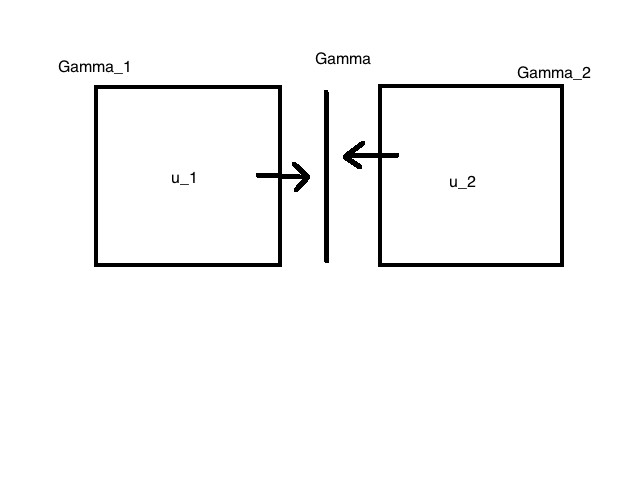
\includegraphics[width=.6\textwidth]{figs/DDdiagram.png}
%\end{figure}

\section{Primal DPG and preconditioning}

The DPG system can be reordered 
\[
A = \left[\begin{array}{c c}
B^TR_V^{-1}B & B^TR_V^{-1}\hat{B}\\
\hat{B}^TR_V^{-1}B & \hat{B}^TR_V^{-1}\hat{B}
\end{array}
\right]\vecttwo{u}{\uh} = \arr{A_h}{B_h}{B_h^T}{C_h}\vecttwo{u}{\uh} = \vecttwo{f_h}{g_h}
\]
where 
\[
\vecttwo{f_h}{g_h} = \vecttwo{B^TR_V^{-1} f}{\hat{B}^TR_V^{-1}f}.
\]
where $A_h$ is the matrix corresponding to field (volume) variables, $C_h$ is the submatrix corresponding to flux (surface/mortar) variables, and $B_h$ couples the system together.  

For a first pass, we consider the primal DPG method, which is probably the simplest DPG method available, where field variables are approximated with $C_0$-continuous piecewise polynomials and the flux variables are approximated using discontinuous mortar basis functions.  Test functions are approximated with disjoint discontinuous polynomials of higher order than the trial field variables.  (We may also wish to consider the DPG method with ultra-weak variational formulation (discontinuous field variables).  In this case, $A_h$ is also block diagonal.)

\subsection{Block Jacobi}

We can write the full DPG system in block form
\[
\arr{A_h}{B_h}{B_h^T}{C_h}\vecttwo{u}{\uh} = \vecttwo{f_h}{g_h}.
\]
We could naively break the system up into two blocks and use a fixed point iterative scheme
\begin{align*}
u^{n+1} &= A_h^{-1}(f_h-B_h\uh^{n})\\
\uh^{n+1} &= C_h^{-1}(g_h-B_h^Tu^{n+1}).
\end{align*}
or equivalently
\[
\vecttwo{u^{n+1}}{\uh^{n+1}} = \arr{A_h^{-1}}{}{}{C_h^{-1}}\LRp{\vecttwo{f_h}{g_h} - \arr{}{B_h}{B_h^T}{}\vecttwo{u^n}{\uh^n}}
\]
which we can recognize as a block Jacobi iteration.  This may be preferrable in a matrix-free environment, as both $A_h$ and $C_h$ can be computed in a matrix-free fashion ($C_h\uh$ can be computed using local inversions of the Riesz product with $\uh$ as boundary data).  As far as I can tell, the Schur complement $S = C_h-B_h^TA_h^{-1}B_h$ for a general DPG system cannot, due to the non-explicit nature of $A_h = B_h^TR_V^{-1}B_h$.

This iteration was tested on pure convection under both the ultra-weak and primal formulations.  As there was no observable difference in the primal formulation, we just show ultra-weak results here.  Test norm was taken to be $\nor{v}_V^2 = \alpha\nor{v}_{\L}^2 + \nor{\beta\cdot\grad v}_{\L}^2$.  
\begin{itemize}
\item Convergence depends on $\Delta N$ and $N_{\rm flux}$.  
\item If $N_{\rm flux} = 0$, convergence is roughly independent of $\Delta N$.  If $N_{\rm flux} > 0$, the convergence is both slower than with $N_{\rm flux} = 0$ and more sensitive to $N$ and $\Delta N$.
\end{itemize}

Convergence of the fixed point solution to the exact solution is shown here.
\begin{figure}
\centering
\subfigure[$N_{\rm flux} = 1, \Delta N = 2$]{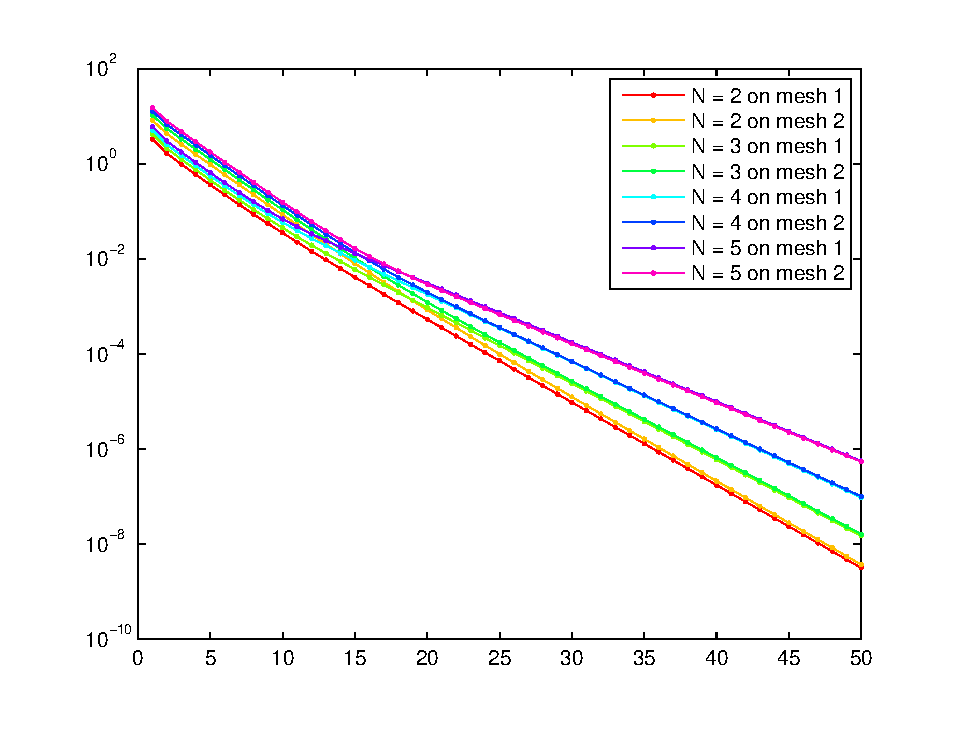
\includegraphics[width=.49\textwidth]{figs/Nflux1_DP2.eps}}
\subfigure[$N_{\rm flux} = 1, \Delta N = 4$]{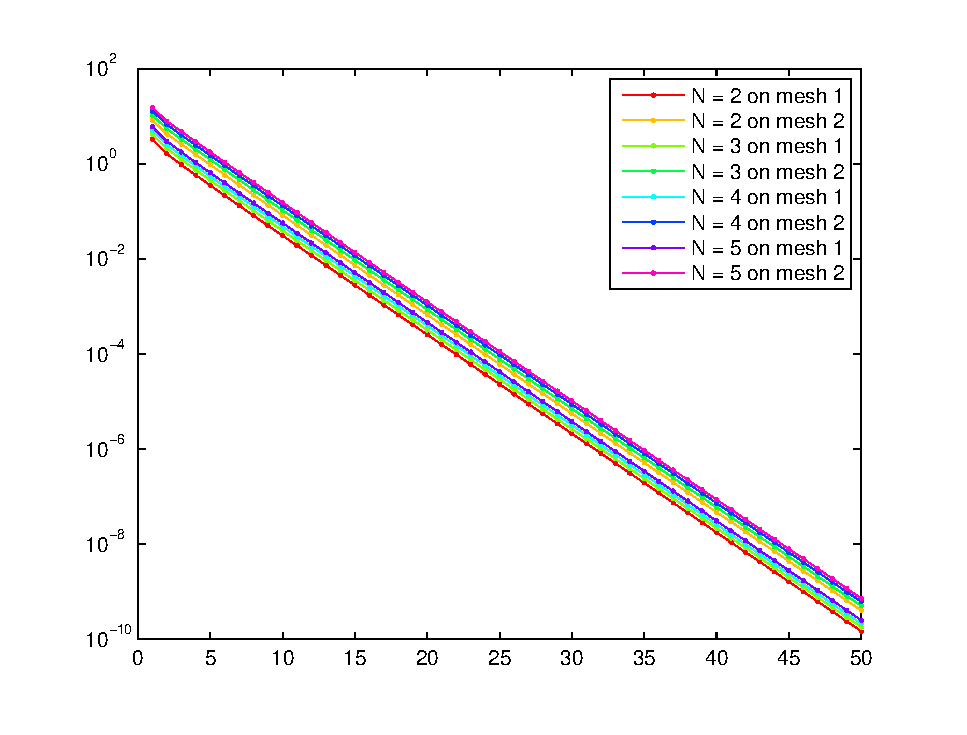
\includegraphics[width=.49\textwidth]{figs/Nflux1_DP4.eps}}
\subfigure[$N_{\rm flux} = 0, \Delta N = 4$]{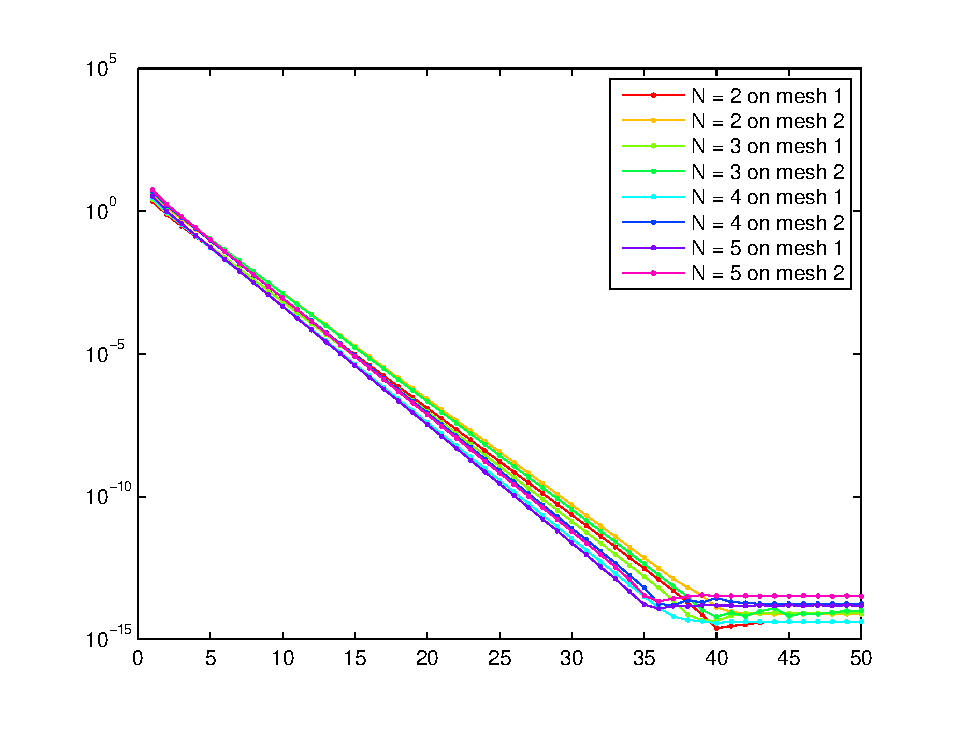
\includegraphics[width=.49\textwidth]{figs/Nflux0_DP2.eps}}
\subfigure[$N_{\rm flux} = 0, \Delta N = 2$]{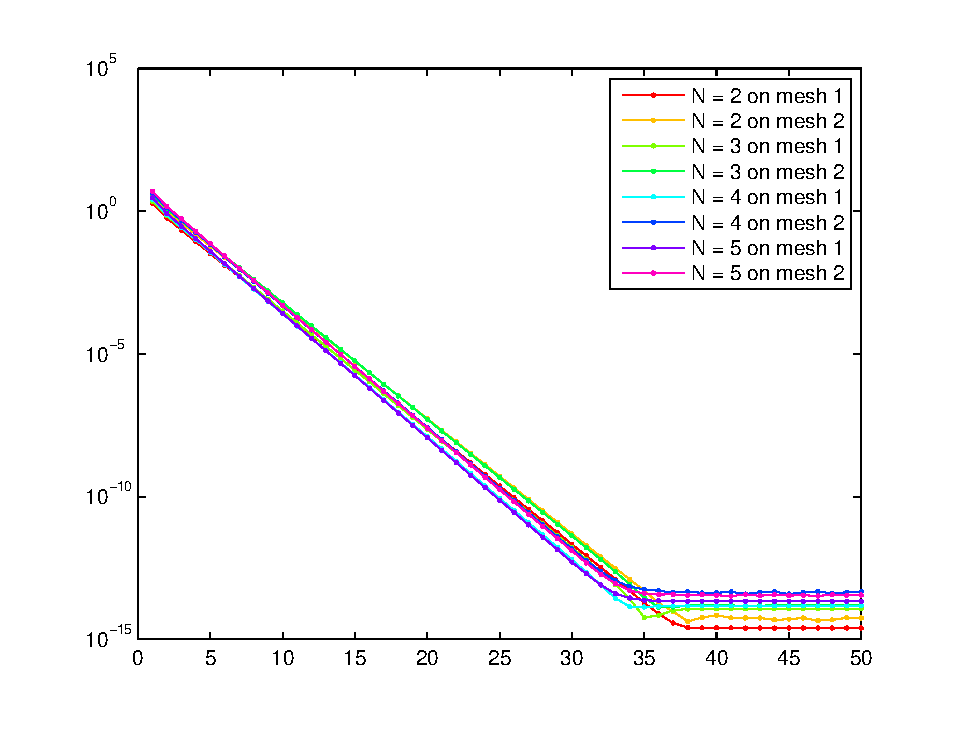
\includegraphics[width=.49\textwidth]{figs/Nflux0_DP4.eps}}
\caption{Block Jacobi fixed point iterations for pure convection with $\beta = (1,0)$, ultra-weak formulation.}
\end{figure}

We note that these results are sensitive also to the regularization parameter $\alpha$ --- smaller $\alpha$ results in faster convergence, but obviously worse conditioning of the local problem.  
\begin{figure}
\centering
\subfigure[$N_{\rm flux} = 0$]{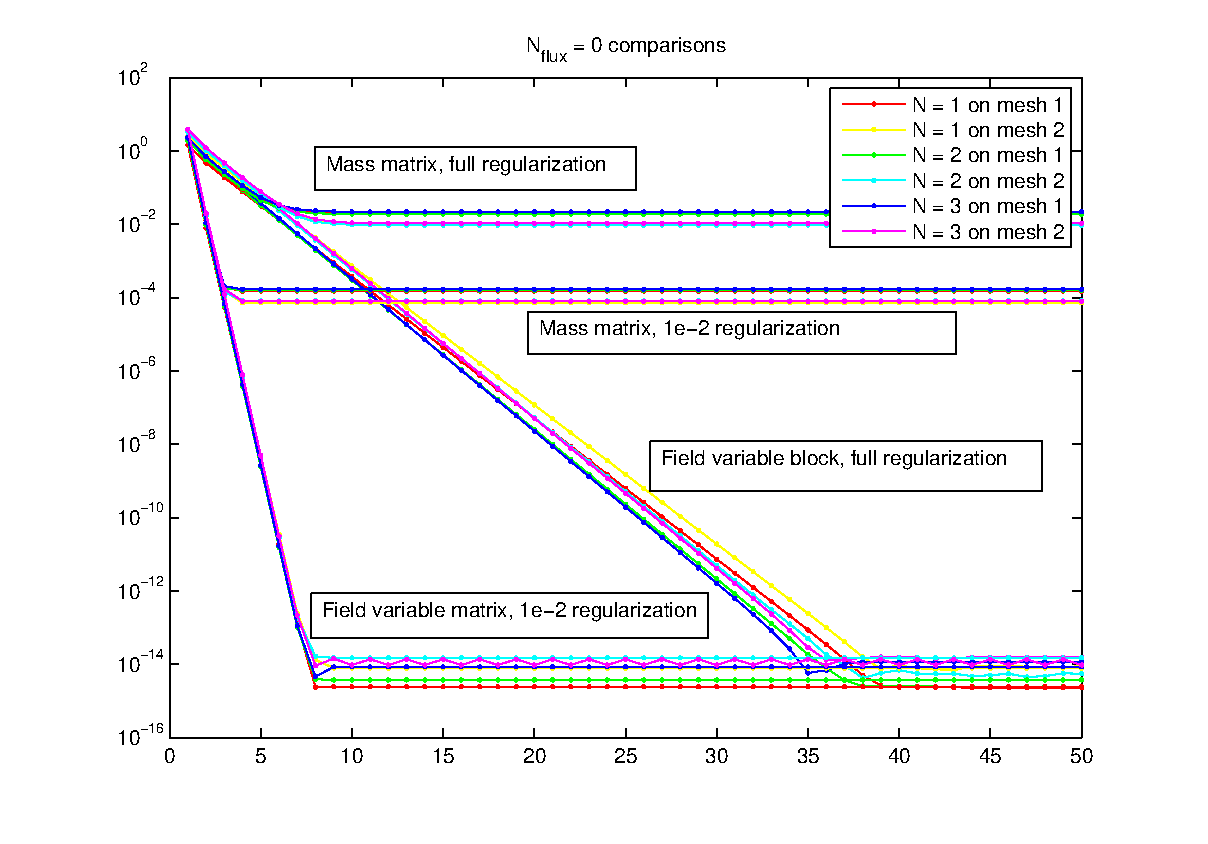
\includegraphics[width=.49\textwidth]{figs/Nflux0_compare.eps}}
\subfigure[$N_{\rm flux} = N_{\rm trial}$]{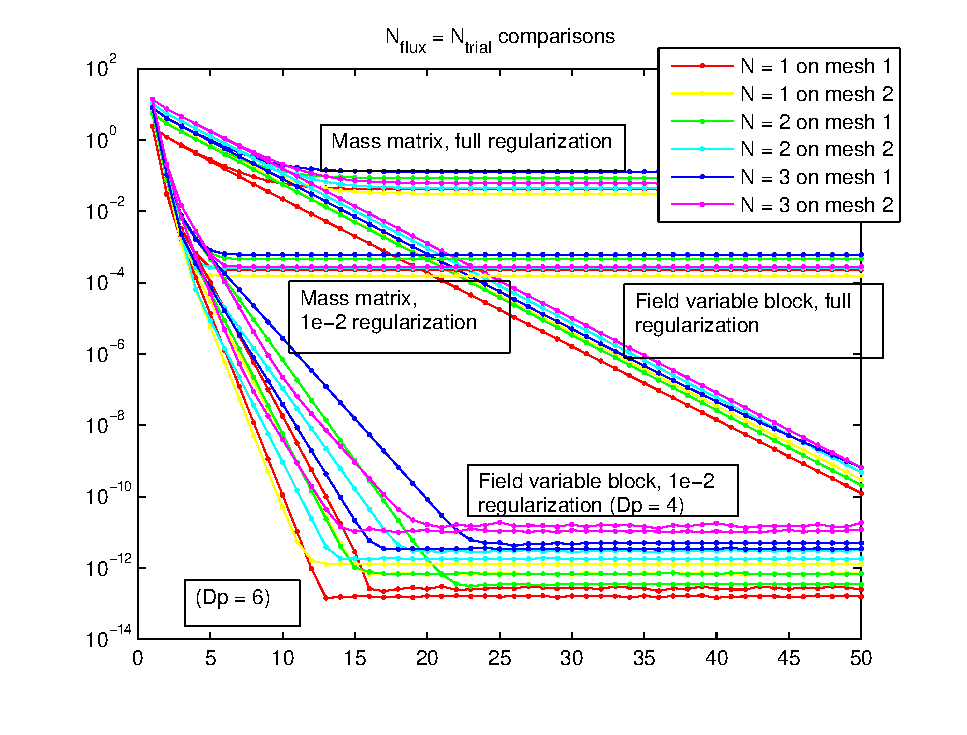
\includegraphics[width=.49\textwidth]{figs/NfluxTrial_compare.eps}}
\caption{Block Jacobi fixed point iterations for pure convection - dependence on $\alpha$ regularization parameter.  ``Mass matrix'' means that the solution of $B^TR_V^{-1}B$ was replaced by the inversion of an $\L$ mass matrix instead.}
\end{figure}

Questions: 
\begin{itemize}
\item Do the results carry over for the ultra-weak formulation?  Maybe only using the graph norm?  
\item Why do these results fail for Poisson's equation in the primal formulation?  
\item \textbf{This has to be related to the fixed point/Uzawa iteration of Dahmen.}  Issues in generalization described below.
\end{itemize}

\section{Issues with this idea}

\begin{itemize}
\item Main problem: for ultra-weak DPG, the matrix 
\[
C = \hat{B}R_V^{-1}\hat{B}
\]
has exactly the same sparsity structure as the Schur complement $S = C - B^TA^{-1}B$ if we take discontinuous trial functions.  The advantage: $C$ is slightly better conditioned in practice, and there are better-known ways to precondition mortar systems.  However, the preconditioner becomes sensitive to tolerances (AGMG needs a lot of iterations/low tolerance to do well in the inner iteration, though it gets better w/$\alpha$ larger).  Do we gain anything else here?  
\item This approach does not work for second order primal DPG methods - if I take $C_0$ basis functions and add diffusion, this approach fails.  We cannot precondition 2nd order $C_0$ DPG with this method.  
\end{itemize}

Main contribution of this work so far: connecting the block Jacobi DPG idea to Dahmen's fixed point iteration scheme for the mixed DPG formulation.  Noting the dependence of fixed point convergence vs conditioning with $\alpha$.  

\subsubsection{Relation to Dahmen fixed point iteration}

Dahmen's fixed point iteration considers solving
\begin{align*}
(e,v)_V + b(u,v) &= l(v) \\
b(\delta u,e) &= 0
\end{align*}
or, in algebraic form
\[
\arr{R_V}{B}{B^T}{}\vecttwo{e}{u} = \vecttwo{f}{0}.
\]
In the case he examined, he solves the strong equation 
\[
Au = f
\]
such that $v^TBu = (u,A^*v)_{\L}$ and $(\delta v)^TR_Vv = (v,\delta v)_V \coloneqq (A^*v,A^*\delta v)_{\L}$.  His fixed point iteration is then
\begin{align*}
e^{n+1} &= R_V^{-1}(f - Bu^n) \\
Mu^{n+1} &= Mu^n + B^Te^{n+1}.
\end{align*}
where $M$ is the standard $\L$ mass matrix.  His key observation is that the Schur complement $B^TR_V^{-1}B$, while completely dense, should converge to $M$ if the test space for $v$ is sufficiently large.  He uses $C_0$ basis functions for the trial space, but could have easily switched to $L^2$ basis functions instead.  

Suppose now that we take the DPG approach to the above iteration.  Then, we can solve for the auxiliary variables $\widehat{u}$ instead of solving for $e$ via the system
\[
\arr{R_V}{\Bh}{\Bh^T}{}\vecttwo{e}{\uh} = \vecttwo{f-Bu}{0}
\]
which yields 
\begin{align*}
\uh &= (\Bh^TR_V^{-1}\Bh)^{-1} \Bh^T R_V^{-1}(f-Bu)\\
e &= R_V^{-1}(f - Bu - \Bh \uh ).
\end{align*}
Supposing $M$ can be replaced by the positive definite matrix $B^TR_V^{-1}B$, we can rewrite Dahmen's iteration as the following: given $u^n$,
\begin{align*}
\uh^n &= (\Bh^TR_V^{-1}\Bh)^{-1} \Bh^T R_V^{-1}(f-Bu^n)\\
e^{n+1} &= R_V^{-1}(f - Bu^n - \Bh \uh ^n) \\
u^{n+1} &= u^n + (B^TR_V^{-1}B)^{-1}B^Te^{n+1}.
\end{align*}
We can eliminate $e^{n+1}$ to arrive at 
\begin{align*}
\uh^n &= (\Bh^TR_V^{-1}\Bh)^{-1} \Bh^T R_V^{-1}(f-Bu^n)\\
u^{n+1} &= (B^TR_V^{-1}B)^{-1}B^TR_V^{-1}(f - \Bh \uh ^n) .
\end{align*}
Substituting in the definitions of $A_h, B_h,$ and $C_h$, we arrive at
\begin{align*}
\uh^n &= C_h^{-1} (g_h - B_h^T u^n)\\
u^{n+1} &= A_h^{-1}(f_h - B_h \uh ^n) 
\end{align*}
which is nothing more than a block Jacobi iteration.  

\subsubsection{Variational crimes}

DPG commits two ``crimes'' compared to Dahmen's work.  
\begin{itemize}
\item Under the graph norm for DPG, we modify $R_V$ to be 
\[
\nor{v}_V^2 = \alpha \nor{v}_{\L}^2 + \nor{A^*v}_{\L}^2.
\]
This makes $R_V$ a positive definite operator.  Dahmen relied on the fact that $R_V$ was invertible only under proper assumptions on the test space (i.e. boundary conditions on $V$).  However, this relies on $R_V$ being global.  

We note that this relies on DPG using the graph norm.  It's not known whether or not equivalent results hold for robust (but non-graph) test norms.  

\item We use the primal hybrid formulation as a nonconforming method to approximate $e$.  $e$ is then condensed out to yield Lagrange multipliers $\uh$, which are appended to the the global system (much like FETI).  However, the condensation yields that the total system is now symmetric positive definite.  
\end{itemize}
Convergence analysis of the Jacobi fixed-point iteration will depend on adapting Dahmen's proof to accomodate these two conditions.  

Conjecture: convergence of the Jacobi scheme is dependent only on optimal test functions for interface unknowns being approximated sufficiently well.  Numerical results indicate that convergence is largely independent of $\Delta p$ or $N$ in the case where $N_{\rm flux} = 0$.  

\subsection{GMRES preconditioner}

An issue with preconditioning using a fixed point iteration is that the preconditioner is no longer symmetric positive-definite, though we can still take advantage of the positive-definite nature of the blocks in the block Jacobi iteration.  We therefore use the block Jacobi iteration as a GMRES preconditioner.  We chart the dependence of the method on $\alpha$ and the number of fixed point iterations below.  
\begin{figure}
\centering
\subfigure[$\alpha = 1$]{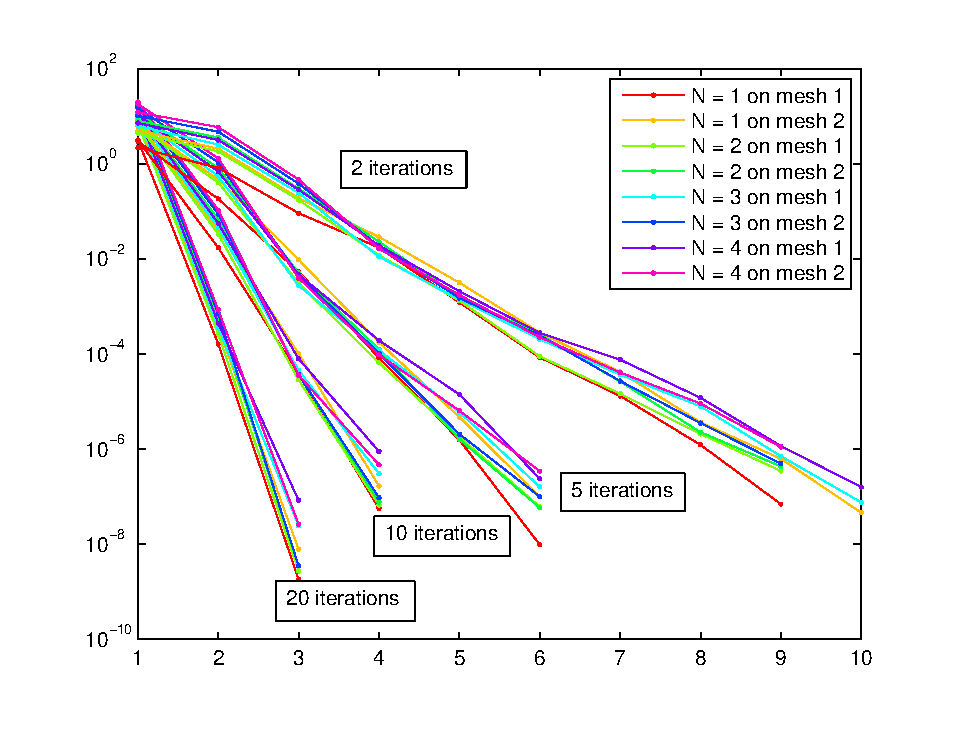
\includegraphics[width=.49\textwidth]{figs/GMRES_bJacobi.eps}}
\subfigure[$\alpha = .1$]{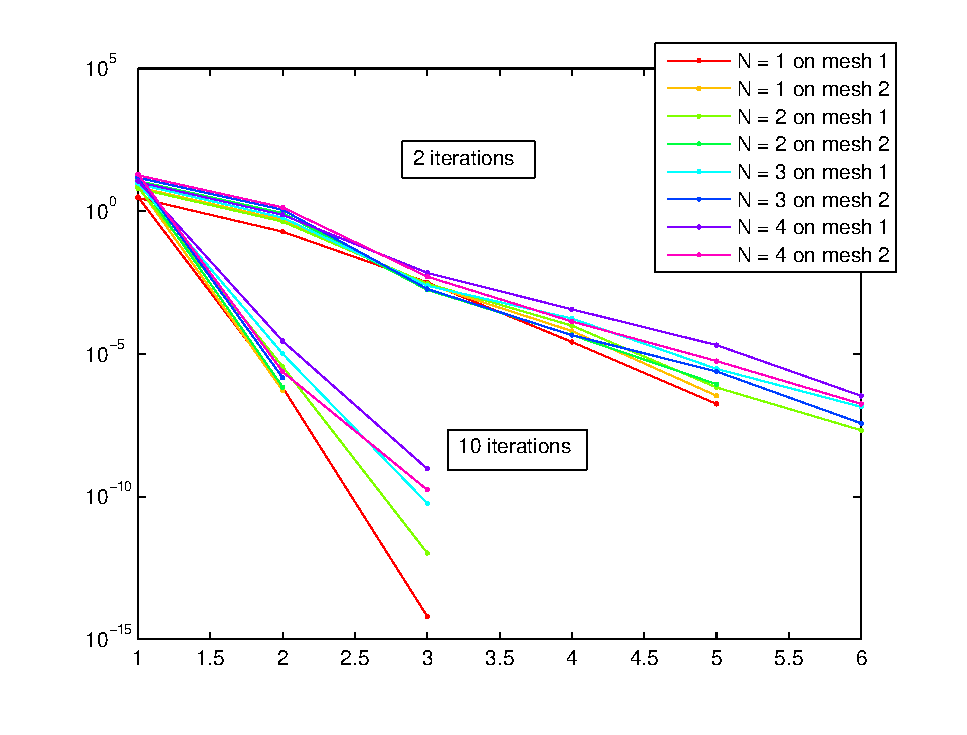
\includegraphics[width=.49\textwidth]{figs/GMRES_bJacobi_alpha10th.eps}}
\caption{Block Jacobi fixed point iterations for pure convection used as a preconditioner for GMRES.}
\end{figure}
Counting the total number of solves in both inner and outer GMRES iterations, we can see that, while a larger number of inner iterations speeds up GMRES convergence, the most efficient method in terms of number of total solves is a single inner iteration.  Thus, we abandon the idea of a fixed point iteration in favor of a single step preconditioner.  Doing so will also allow us to construct a symmetric, positive-definite preconditioner for use in a conjugate gradient iteration.  

\section{Block triangular factorization vs fixed point iteration}

We can do a block triangular factorization of this system 
\[
A = \arr{I}{0}{B_h^TA_h^{-1}}{I}\arr{A_h}{0}{0}{S}\arr{I}{A_h^{-1}B_h}{0}{I}.
\]
where $S = C_h - B_h^TA_h^{-1}B_h$, the Schur complement.  The inverse can be explicitly written
\[
A^{-1} = \arr{I}{-A_h^{-1}B_h}{0}{I}\arr{A_h^{-1}}{0}{0}{S^{-1}}\arr{I}{0}{-B_h^TA_h^{-1}}{I}
\]
Preconditioners based on this factorization often involve an approximation of the Schur complement, which, in this case, is
\[
S = \hat{B}^TR_V^{-1}\hat{B} - \hat{B}^TR_V^{-1}{B}\LRp{B^TR_V^{-1}B}^{-1} B^TR_V^{-1}\hat{B}
\]
%Factoring out $\hat{B}$ on both sides gives
%\[
%S = \hat{B}^T\LRp{R_V^{-1} - R_V^{-1}{B}\LRp{B^TR_V^{-1}B}^{-1} B^TR_V^{-1}}\hat{B}
%\]
%Factoring out $\hat{B}^TR_V^{-1}$ on both the left and right gives
%\[
%S = \hat{B}^TR_V^{-1}\LRp{R_V-B\LRp{B^TR_V^{-1}B}^{-1}B^T}R_V^{-1}\hat{B}
%\]
%If we define $\tilde{B} = R_V^{-1/2}{B}$, then the above is
%\[
%S = \hat{B}^TR_V^{-1/2}\LRs{I - \tilde{B}(\tilde{B}^T\tilde{B})^{-1}\tilde{B}^T}R_V^{-1/2}\hat{B}.
%\]
%The matrix $\LRs{I - \tilde{B}(\tilde{B}^T\tilde{B})^{-1}\tilde{B}^T}$ is the orthogonal projector onto the kernel of $\tilde{B}^T$ - does this help? 
Suppose we just wish to precondition $S$ with $C = \hat{B}^TR_V^{-1}\hat{B}$.  This assumes that $C^{-1}S = I - C^{-1}B^TA^{-1}B$ is close to an identity, or that $C^{-1}B^TA^{-1}B$ is nearly zero.  Numerical experiments with Poisson/convection-diffusion indicate this may holds independently of $h$, though convection-diffusion appears to have dependence on $N$ for $N>4$ and $\epsilon \ll 1$ or $\epsilon \gg 1$.  

Suppose we apply just the rightmost two matrices to the DPG right hand side; we get
\[
\vecttwo{u^{n}}{\uh^{n+1}} = \arr{A_h^{-1}}{0}{0}{C_h^{-1}}\arr{I}{0}{-B_h^TA_h^{-1}}{I}\vecttwo{f_h}{g_h} = \vecttwo{A_h^{-1}f_h }{C_h^{-1}(g_h - B_hA_h^{-1}f_h)}= \vecttwo{A_h^{-1}f_h }{C_h^{-1}(g_h - B_hu^{n})}
\]
which we can recognize as one iteration of block Jacobi starting with $u^{n} = A_h^{-1}f_h$ and $\uh^n = 0$.  An application of the leftmost matrix then gives
\[
\arr{I}{-A_h^{-1}B_h}{0}{I}\vecttwo{A_h^{-1}f_h }{C_h^{-1}(g_h - B_hu^{n+1})} = \vecttwo{A_h^{-1}(f_h - B_h \uh^{n+1})}{\uh^{n+1}} = \vecttwo{u^{n+1}}{\uh^{n+1}}.
\]
Thus, an application of this preconditioner is equivalent to a single symmetric application of the fixed point iteration.  

Preliminary results applied to Poisson ($\beta = 0, \epsilon = 1$) and convection-diffusion are given below.  
\begin{figure}
\centering
\subfigure[Poisson]{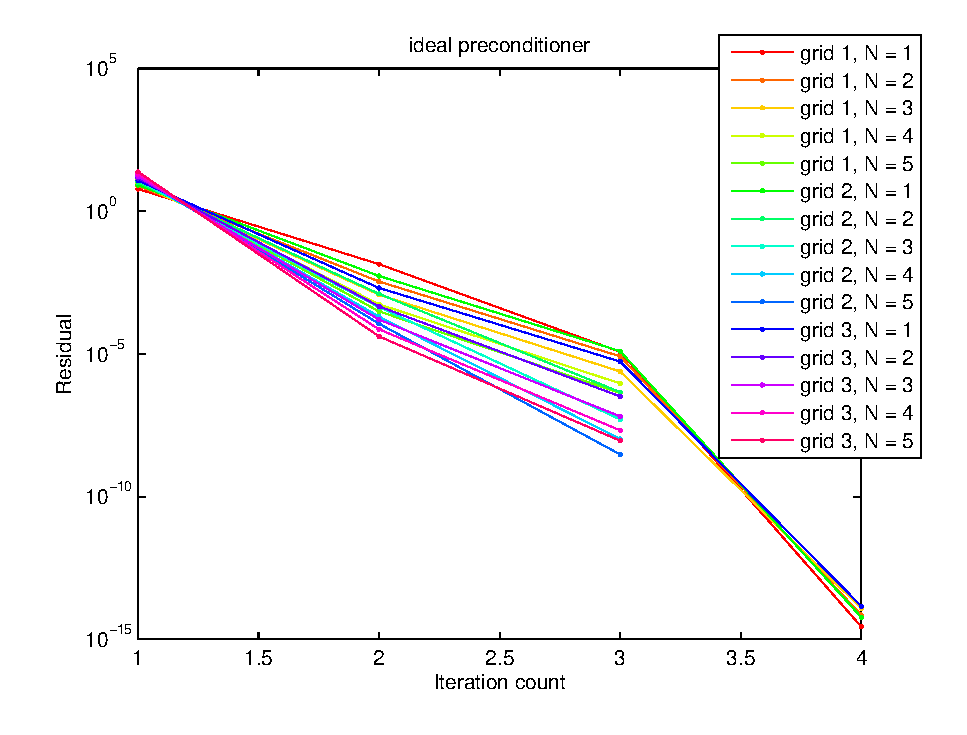
\includegraphics[width=.49\textwidth]{figs/ideal_poisson.eps}}
\subfigure[Convection-diffusion, $\epsilon = 10^{-1}$]{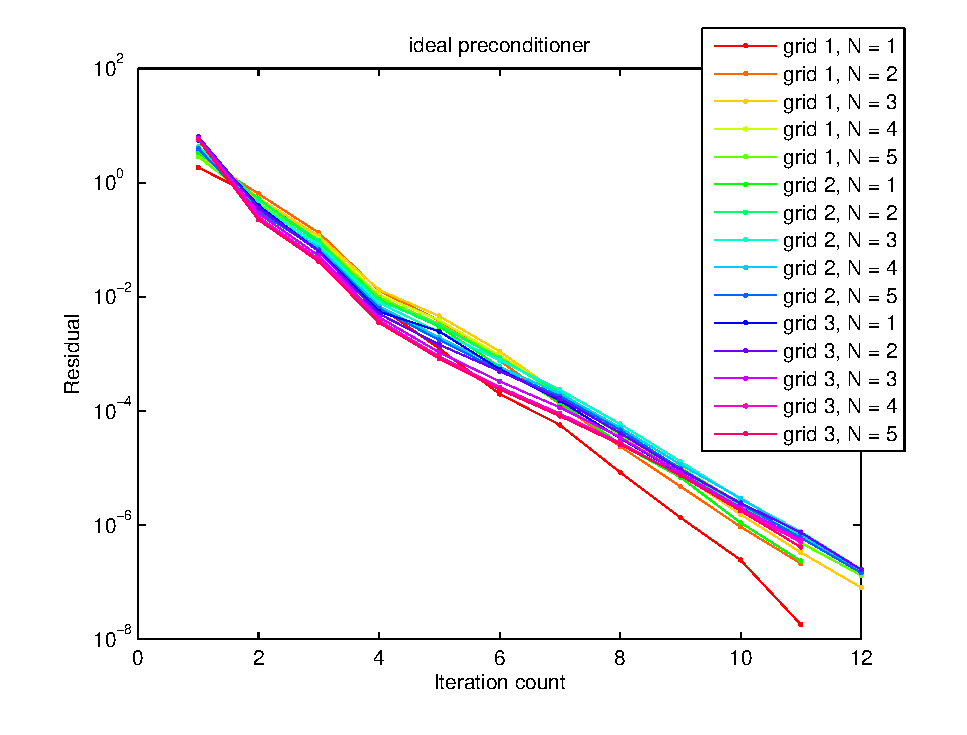
\includegraphics[width=.49\textwidth]{figs/ideal_confusion1e1.eps}}
\caption{Triangular factorization preconditioners for Poisson and diffusion-dominated convection-diffusion.}
\end{figure}

Convergence of convection-diffusion suffers at higher $N$ when diffusion is taken to be $10^{-3}$; however, it recovers again when $\epsilon = 10^{-6}$.  At very small $\epsilon$, $A_h = B^TR_V^{-1}B \approx M$ again, and convergence of the fixed-point iteration is very fast.  
\begin{figure}
\centering
\subfigure[Convection-diffusion, $\epsilon = 10^{-3}$]{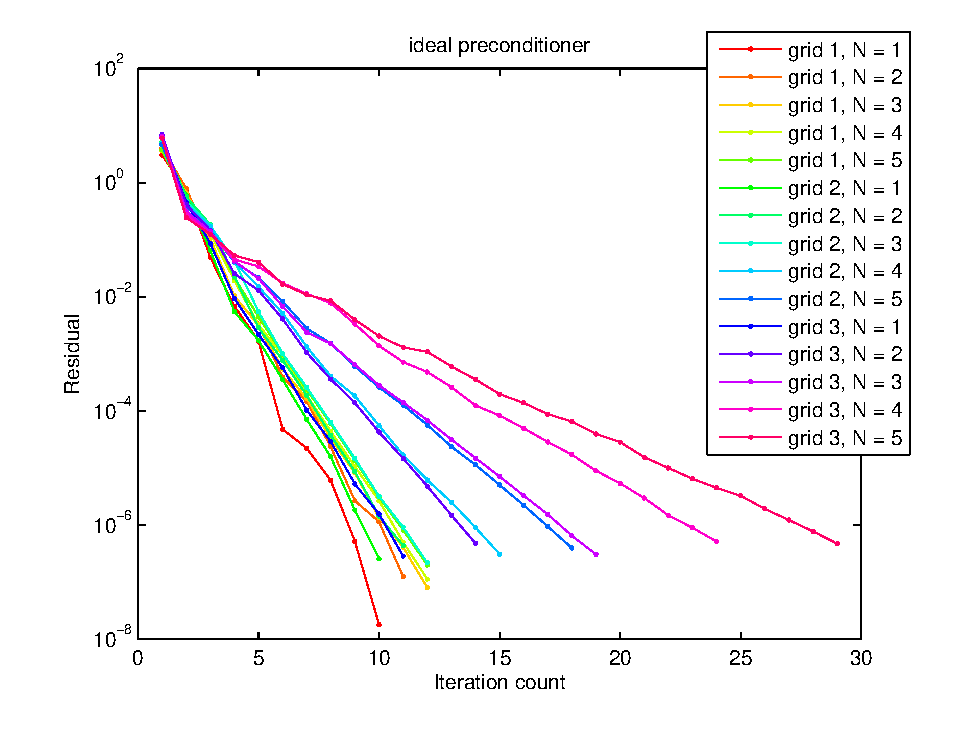
\includegraphics[width=.49\textwidth]{figs/ideal_confusion1e3.eps}}
\subfigure[Convection-diffusion, $\epsilon = 10^{-6}$]{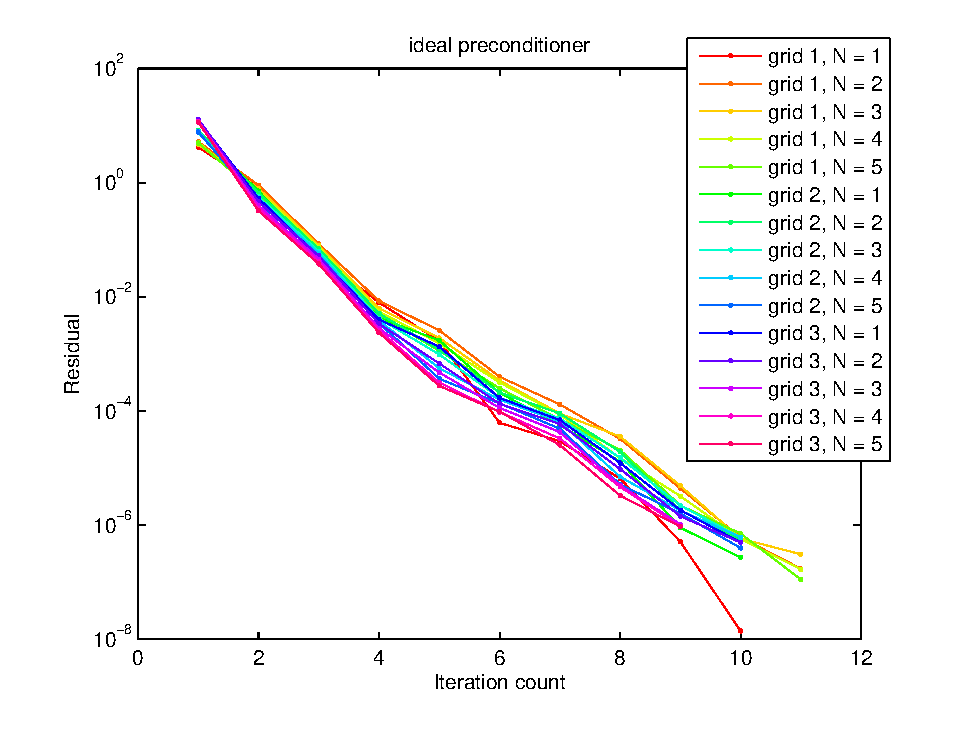
\includegraphics[width=.49\textwidth]{figs/ideal_confusion1e6.eps}}
\caption{Triangular factorization preconditioner for convection-diffusion.}
\end{figure}

\subsection{Approximate inverses}

We assume that preconditioning the $A_h$ submatrix can roughly be done using similar techniques to preconditioning standard elliptic equations.  Initial numerical evidence appears to support this.  Options include 
\begin{itemize}
\item Two-level additive Schwarz.  A coarse solve ($P_1$ elements with AGMG?) + (overlapping) block solves.  \textcolor{red}{Not working yet.}
\item Direct AGMG preconditioning.  \textcolor{red}{Working for CG and DPG.}
\item $P_1$ FEM preconditioning of nodal bases \textcolor{red}{Working for CG, not yet implemented for DPG.}
\item Geometric multigrid.  
\end{itemize}

Preconditioning of the $C_h$ submatrix is more difficult conceptually; however, similar ideas can be leveraged
\begin{itemize}
\item Two-level additive Schwarz.  A coarse solve ($P_1$ elements with AGMG?) + (overlapping) block solves.  \textcolor{red}{Not working yet.}
\item Direct AGMG preconditioning
\item Geometric multigrid.  
\end{itemize}
$P_1$ FEM preconditioning is meant to sparsify the structure of the finite element matrix; however, since the $C_h$ submatrix is constructed in a Schur complement manner, replacing a nodal polynomial on an edge would not 


\subsection{Etc notes}
\begin{itemize}
\item Can we use the idea of reducing to field dofs?  i.e. turn the inversion of the flux matrix into just an outer product?  Make equiv to testing with null space of $\hat{B}^T$...
\item Can we change the coupling to the mortar space for $e$?  i.e. add consistency/penalty/etc?
\item Try boundary penalization in test norms.  
\end{itemize}

\end{document}

